\subsection{Modellbildung}
\label{subsec:02modellbildung}
Um eine Beziehung zwischen physikalischer Gr\"o\ss{}e f\"ur Geschwindigkeit und Lenkwinkel und der entsprechenden Stellgr\"o\ss{}e zu herzustellen, wird jeweils ein Modell ben\"otigt.
\paragraph{Geschwindigkeitsmodell} 
Die Daten aus Abbildung \ref{fig:Geschwindigkeitsmodell} wurden bei einer Messfahrt mit Hilfe eines rosbag aufgezeichnet und im Anschluss mit dem Tool plotjuggler ausgewertet. Dazu wurde das Fahrzeug mit Geschwindigkeitsstellgr\"o\ss{}en im Intervall von $-500$ bis $1000$ angesteuert und die jeweilige Geschwindigkeit aus der Odometrie ausgelesen. Auff\"allig ist der Sprung am Achsenursprung, der dadurch entsteht, dass das Fahrzeug eine bestimmte Stellgr\"o\ss{}e ben\"otig, um seine Tr\"agheit zu \"uberwinden.
Die gemessenen Daten lassen sich durch zwei Gerade approximieren:
\begin{align*}
  f(x) =
  \begin{cases}
  439.8038\cdot x+116.136943 & \text{f\"ur } x < 0 \\
  0 & \text{f\"ur } x=0\\
  477.518514\cdot x-104.623299 & \text{f\"ur } x > 0 
  \end{cases}
\end{align*}

\begin{figure}[h]
	\centering
	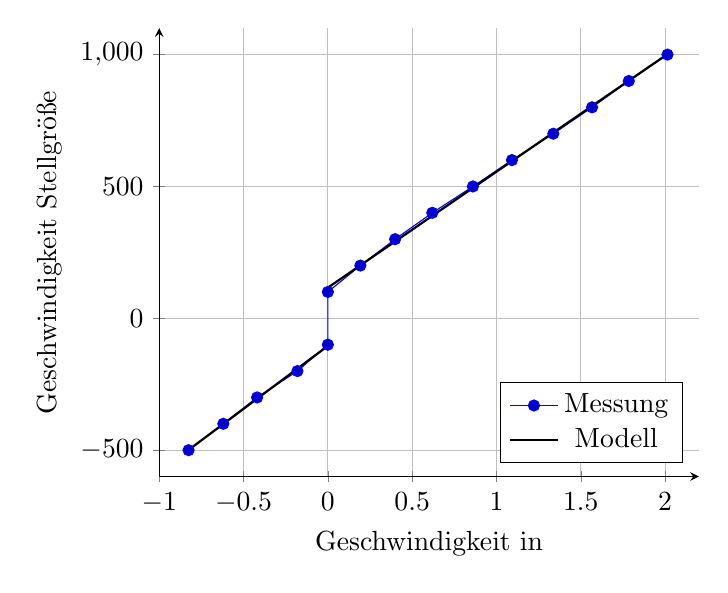
\begin{tikzpicture}
	\begin{axis}[xlabel = Geschwindigkeit in \si{\meter\per\second},ylabel=Geschwindigkeit Stellgr\"o\ss{}e,xmin=-1,xmax=2.2,ymin=-600, ymax=1100, restrict y to domain=-1000:1000,axis x line=bottom, axis y line	=left,grid,legend pos=south east]
	\addplot coordinates  {
		(-0.825872,	-500)
		(-0.619982,	-400)
		(-0.419542,	-300)
		(-0.180354,	-200)
		(0,	-100)
		(0,	100)
		(0.19274,	200)
		(0.398807,	300)
		(0.619379,	400)
		(0.860194,	500)
		(1.091549,	600)
		(1.337146,	700)
		(1.566767,	800)
		(1.784505,	900)
		(2.013835,	1000)
		};
	\addlegendentry{Messung}
	
	\addplot[samples=300,thick,domain=0:2.013835] {439.8038*x+116.136943};
	\addplot[samples=300,thick,domain=-0.825872:0] {477.518514*x-104.623299};
	\addlegendentry{Modell}
	\end{axis}
	\end{tikzpicture}
	\caption{Messung und Geschwindigkeitsmodell.}
	\label{fig:Geschwindigkeitsmodell}
\end{figure}

\paragraph{Lenkwinkelmodell}
Die Bestimmung des Lenkwinkelmodells (Abbildung \ref{fig:Lenkwinkelmodell}) erfolgte nach dem Schema:
\begin{itemize}
	\item Auto anheben und Stellgr\"o\ss{}e f\"ur den Lenkwinkel auf 0 setzen
	\item Mit Geschwindigkeit 300 kurz geradeaus fahren und dann Lenkwinkel einstellen
	\item Geschwindigkeit auf 0 setzen und den Lenkwinkel mit einem Geodreieck messen
\end{itemize}
Dazu war das Paket rqt\_reconfigure sehr hilfreich. Die gemessenen Daten wurden im Anschluss durch das Polynom sechsten Grades
\begin{align*}
196814\cdot x^6 - 50518\cdot x^5 - 47550\cdot x^4 + 5979.7\cdot x^3 + 2459.5\cdot x^2 - 2442.1\cdot x + 143.78
\end{align*} 
approximiert.
Auff\"alig ist die Verschiebung auf der y-Achse, die durch Offset in der Lenkung entsteht. Es sei angemerkt, dass die Messungen mit Fehlern behaftet waren und somit eine ungenaues Lenkwinkelmodell entstanden ist. Genauere Ergebnisse k\"onnte man mit Verwendung der Odometrie bei einer Fahrt im Kreis erzielen.
\begin{figure}[h]
	\centering
	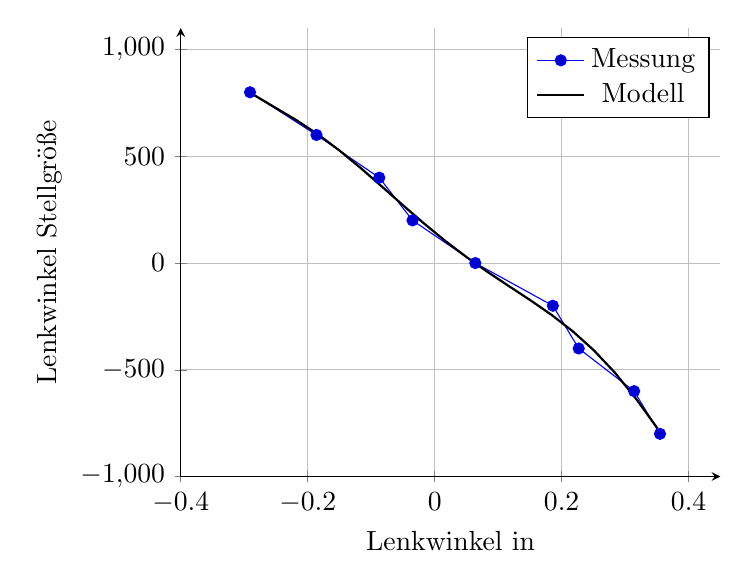
\begin{tikzpicture}
	\begin{axis}[xlabel = Lenkwinkel in \si{\radian},ylabel=Lenkwinkel Stellgr\"o\ss{}e,xmin=-0.40,xmax=0.45,ymin=-1000, ymax=1100, restrict y to domain=-800:800,axis x line=bottom, axis y line	=left,grid]
	\addplot coordinates  {
		(0.3548836146,-800)
		(0.3141592654,-600)
		(0.2268928028, -400)
		(0.1861684535, -200)
		(0.0639954059, 0)
		(-0.034906585, 200)
		(-0.0872664626, 400)
		(-0.1861684535, 600)
		(-0.2908882087, 800)};
	\addlegendentry{Messung}
	
	\addplot[samples=300,thick] {196814*x^6 - 50518 * x^5 - 47550 * x^4 + 5979.7 * x^3 + 2459.5 * x^2 - 2442.1 * x + 143.78};
	\addlegendentry{Modell}
	\end{axis}
	\end{tikzpicture}
	\caption{Messung und Lenkwinkelmodell.}
	\label{fig:Lenkwinkelmodell}
\end{figure}